%
% LaTeX report template 
%

% This is a comment: in LaTeX everything that in a line comes
% after a "%" symbol is treated as comment

\documentclass[11pt, a4paper]{article}
\usepackage{graphicx}
\usepackage{amsmath}
\usepackage{listings}
\usepackage{color}
%\usepackage{fancyvrb} 

\definecolor{dkgreen}{rgb}{0,0.6,0}
\definecolor{gray}{rgb}{0.5,0.5,0.5}
\definecolor{mauve}{rgb}{0.58,0,0.82}

\lstset{frame=tb,
  language=Python,
  aboveskip=3mm,
  belowskip=3mm,
  showstringspaces=false,
  columns=flexible,
  basicstyle={\small\ttfamily},
  numbers=none,
  numberstyle=\tiny\color{gray},
  keywordstyle=\color{blue},
  commentstyle=\color{dkgreen},
  stringstyle=\color{mauve},
  breaklines=true,
  breakatwhitespace=true,
  tabsize=3
}
\title{Assignment No 3} % Title

\author{Manvar Nisharg \\ {\small EE19B094}}

\date{01-03-2021} % Date for the report
\begin{document}		
		
\maketitle % Insert the title, author and date
\section{Abstract}
%Create new section;it is autonumbered
\par The main aim of this assignment is to learn data fitting and study the effect of different level of noise on data fitting. We use data points generated from Bessel function with varying noise(Gaussian's with different $\sigma$). We plot different graphs and analyse the relationship between error in estimations of parameters (mainly A and B) with change of $\sigma$.\\

\section{Introduction}
We generate 10 columns of data of which first column represents time and the rest nine are data points at those time values but with varying noise.\\

The functions used is a linear combination of Bessel Function of first kind and time.\\If n(t) is the noise function with a given $\sigma$ then:\\
\begin{equation*}
f(t) = A*J_{2}(t) + B*t + n(t)
\end{equation*}
\\
where A = 1.05 and B = -0.105 are constants and the Probability Distribution Function of noise is given by

 \begin{equation*}
Pr(n(t)|\sigma) = \frac{1}{\sigma\sqrt{2\pi}}exp(\frac{-n(t)^2}{2\sigma^2})
\end{equation*}
\\where $\sigma$ is given by 
\begin{verbatim}
    variance = logspace(-1,-3,9)
\end{verbatim}
and thus noise is assumed to be normally distributed.\\


\section{Tasks}
\subsection{Generation and Loading of Data}
\par Using \emph{generate.py} we create \emph{fitting.dat} data file which contains 10 coloums. First coloumn represents value of time and the remaining nine are function values at the specific time but with varying amount of noise. It is loaded into the python file using \verb|numpy.loadtxt()| function.

\begin{lstlisting}
#Function to load file and generate X and Y matrix
def load_file(file_name):
	try:
		data_matrix = np.loadtxt(file_name)
	except:
		print("Can't load file")
		exit()
	x_matrix = data_matrix[:,0]
	y_matrix = data_matrix[:,1:]
	return x_matrix,y_matrix

#main
x_matrix,y_matrix = load_file("fitting.dat")
\end{lstlisting}

\subsection{Plotting of raw data}
\par We plot the all the data points with varying noise alongside the true value i.e. with no noise using Matplotlib's pyplot library.
\begin{lstlisting}
#Function to plot raw data
def plot_noised_data(x_matrix,y_matrix):
	plt.figure(0)
	for i in range(1,10,1):
		plt.plot(x_matrix,y_matrix[:,i-1],label=r'$\sigma_{%d}$ = %.3f'%(i,variance[i-1]))
	plt.title('Q4:Data to be fitted to theory')
	plt.ylabel(r'$f(t)\ +\ noise \longrightarrow$',size=12)
	plt.xlabel(r't$\longrightarrow$',size=12)
	plt.legend()

#Function to calulate true value for given X matrix
def g(t,A,B):
	return A*sp.jn(2,t)+(B*t)

#Fumction to plot true function
def plot_true_graph(x_matrix):
	plt.figure(0)
	plt.grid(True)
	plt.plot(x_matrix,g(x_matrix,Ao,Bo),label='True Value')
	plt.legend()
	plt.show()

#main
plot_noised_data(x_matrix,y_matrix)
plot_true_graph(x_matrix)
\end{lstlisting}
\begin{figure}[!tbh]
   	\centering
   	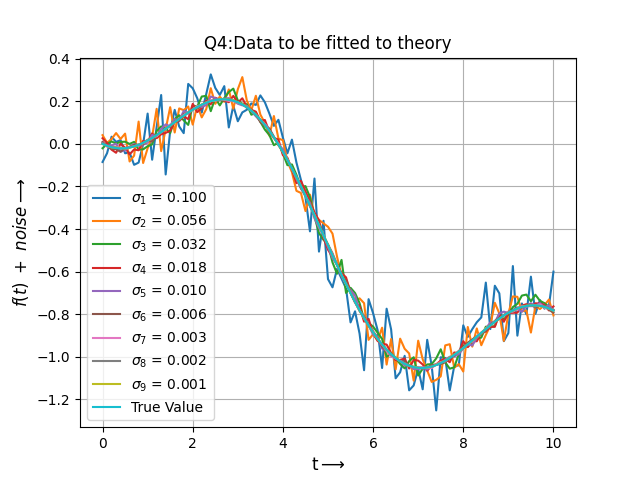
\includegraphics[scale=0.7]{Q3.png}  % Mention the image name within the curly braces. Image should be in the same folder as the tex file. 
   	\caption{Various Functions}
   	\label{fig:Data plot}
   \end{figure} 

\subsection{Error plots}
We visualise the error in the measurement using the \verb|errorbar()| function.
The graph has been obtained by plotting the first column in the data file which corresponds to $sigma = 0.1$\\
The true value has also been plotted for reference.
Here I am plotting the error bar for one data column:\\
\begin{lstlisting}
#Function to plot error bar graph for given error coloumn in Y matrix
def plot_error_bar(x_matrix,y_matrix,coloumn):
	plt.figure(1)
	plt.grid(True)
	plt.plot(x_matrix,g(x_matrix,Ao,Bo),label='True Value')
	plt.errorbar(x_matrix[::5],y_matrix[::5,coloumn],variance[coloumn],fmt='ro', label='errorbar')
	plt.title(r'Q5: Data points for $\sigma = %.3f$ along with exact function'%variance[coloumn])
	plt.xlabel(r't$\longrightarrow$',size=12)
	plt.legend()
	plt.show()

#main
plot_error_bar(x_matrix,y_matrix,0)
\end{lstlisting}
\begin{figure}[!tbh]
   	\centering
   	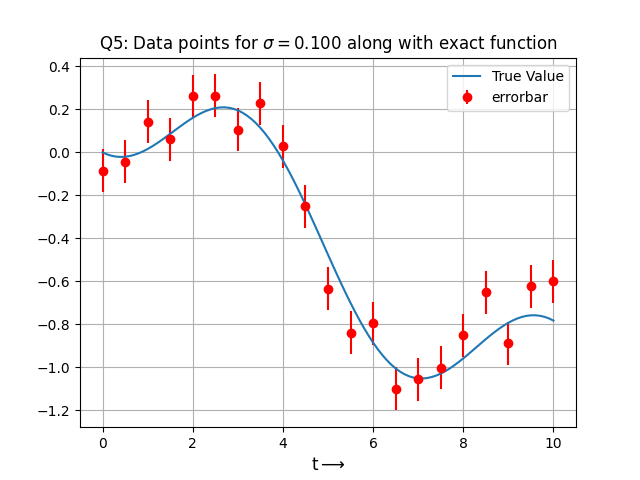
\includegraphics[scale=0.7]{Q5.png}  % Mention the image name within the curly braces. Image should be in the same folder as the tex file. 
   	\caption{Error bars for $\sigma$ = 0.1 along with exact function}
   	\label{fig:Error bar}
   \end{figure}
   

\subsection{Matrix Generation}
\par If we write the equations satisfying the data points in matrix form for general parameters,
%\begin{equation}

\begin{center}
     $   g(t,A,B) = 
    \begin{pmatrix}
    J_{2}(t_{1})& t_{1}\\
    J_{2}(t_{2}) & t_{1}\\
    ... & ...\\
    J_{2}(t_{n})& t_{n}
    \end{pmatrix}
     \begin{pmatrix}
        A \\
        B
    \end{pmatrix} = M\cdot p$
    
\end{center}
\par Thus we generate the  M matrix and check that the true values (using the \verb|g()| funtion) satisfies the Ao and Bo value.
\begin{lstlisting}
#Function to generate M matrix
def generate_M(x_matrix):
	vector1 = sp.jn(2,x_matrix)
	M = np.c_[vector1,x_matrix]
	return M

#main
M = generate_M(x_matrix)
p = np.array([Ao,Bo])
answer = np.matmul(M,p)
g_vector = g(x_matrix,Ao,Bo)
if (answer==g_vector).all():
	print("They are equal")
\end{lstlisting}
%\end{equation}
    

\subsection{MS Error for varying A and B}
We know that the true values satisfies the equation of the form:\\
\begin{equation*}
g(t,A,B) = AJ_{2}(t)+Bt 
\end{equation*}
Our aim is to find appropriate vales of A and B so that given data best fits into the equation.\\\\Thus we vary our values of A and B within an appropriate range and generate a matrix with MS error ($\epsilon_{ij}$) between the data (1st column in our case) and the assumed model for a given $A_i$ and $B_j$
\begin{equation}
    \epsilon_{ij} =  \frac{1}{101}\sum_{k=0}^{101}(f(x)-g(t_k,A_i,B_j))^2
\end{equation}
\begin{lstlisting}
#Function to generate ME matrix
def generate_error_matrix(A_vector,B_vector,x_matrix,y_matrix_coloumn):
	mean_sq_error = np.zeros((np.size(A_vector),np.size(B_vector)))

	row = 0
	for A in A_vector:
		coloumn = 0
		for B in B_vector:
			temp_g = g(x_matrix,A,B)

			error = 0
			for index in range(np.size(x_matrix)):
				error += (y_matrix[index][y_matrix_coloumn]-temp_g[index])**2

			mean_sq_error[row][coloumn] = error/np.size(x_matrix)

			coloumn += 1
		row += 1

	return mean_sq_error

#main
A_vector = np.arange(0,2.1,0.1)
B_vector = np.arange(-0.2,0.001,0.01)
mean_sq_error = generate_error_matrix(A_vector,B_vector,x_matrix,0)
\end{lstlisting}

\subsection{Contour plots for MS error}
\par We can plot the contour plot of MS error for varying A and B. Also the true value of A (i.e. Ao) and B (i.e. Bo) is shown.
\begin{lstlisting}
#Function to plot contour plot of ME matrix
def plot_contour_plots(A_vector,B_vector,mean_sq_error):
	plt.figure(2)
	plt.title(r'Q8: Contour plot of $\epsilon_{ij}$')
	plt.xlabel(r'A$\longrightarrow$',size=12)
	plt.ylabel(r'B$\longrightarrow$',size=12)
	contour_plot = plt.contour(A_vector,B_vector,mean_sq_error,levels=np.arange(0,20*0.025,0.025))
	plt.clabel(contour_plot,contour_plot.levels[:6],inline=True,fontsize=10)
	plt.plot(Ao,Bo,'ro')
	plt.annotate("True Value", (Ao, Bo))
	plt.show()

#main
plot_contour_plots(A_vector,B_vector,mean_sq_error)
\end{lstlisting}

Contour Plot of $MS\ error$ for range of (A,B):
\begin{figure}[!tbh]
   	\centering
   	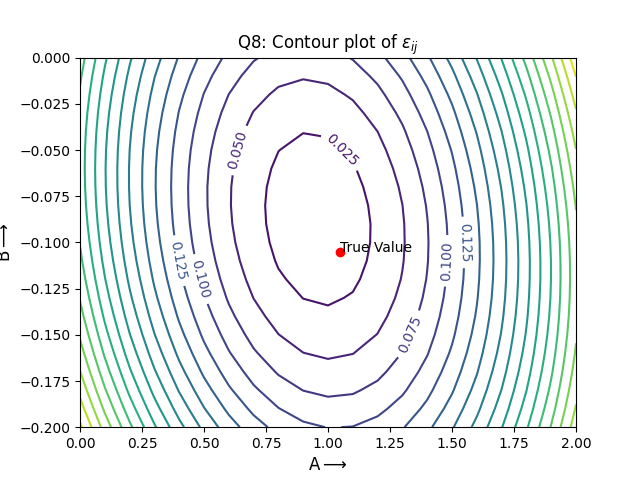
\includegraphics[scale=0.7]{Q8.png}  % Mention the image name within the curly braces. Image should be in the same folder as the tex file. 
   	\caption{contour plot for $\epsilon_{ij}$ }
   	\label{fig:Contour plot}
   \end{figure}
From the above plot we can clearly see that there exist a single minimum.


\subsection{Estimations}
\par Now, we can find the values of A and B by minimizing $|M*(AB)-C|$ where C is one of the columns of data. We can do this using the \verb|scipy.linalg.lstsq()| function.\\
Thus, we find A and B values for each column of data and store it in a list.
\begin{lstlisting}
#Function to predict parameters using lstsq() function for given coloumn
def predict_parameters(M,y_matrix,coloumn):
	predicted_parameters,_,_,_ = scipy.linalg.lstsq(M,y_matrix[:,coloumn])
	return predicted_parameters

#main
predicted_parameters = np.zeros((np.size(y_matrix[0,:]),2))
for coloumn in range(9):
	predicted_parameters[coloumn] = predict_parameters(M,y_matrix,coloumn)
\end{lstlisting}

\subsection{Error plots for different scales}
\par Now, for the above calculated A and B, we find the absolute error between the calculated and the true values and plot them in 2 formats.\\

\subsubsection{Linear scale}
We plot the graph of error with changing values of $sigma_{n}$
\begin{lstlisting}
#Function to plot error in linear scale
def plot_error_plot(p,predicted_parameters):
	plt.figure(3)
	plt.grid(True)
	plt.title(r'Q10: Variation of error with noise')
	plt.xlabel(r'Noise standard deviation$\longrightarrow$')
	plt.ylabel(r'Error$\longrightarrow$')
	error_A = np.zeros(np.size(predicted_parameters[:,0]))
	error_B = np.zeros(np.size(predicted_parameters[:,0]))
	for row in range(np.size(predicted_parameters[:,0])):
		error_A[row] = abs(p[0]-predicted_parameters[row][0])
		error_B[row] = abs(p[1]-predicted_parameters[row][1])
	plt.plot(variance,error_A,'ro-',label='Aerr',linestyle='dotted')
	plt.plot(variance,error_B,'bo-',label='Berr',linestyle='dotted')
	plt.legend()
	plt.show()

	return error_A,error_B

#main
error_A,error_B = plot_error_plot(p,predicted_parameters)
\end{lstlisting}

\begin{figure}[!tbh]
   	\centering
   	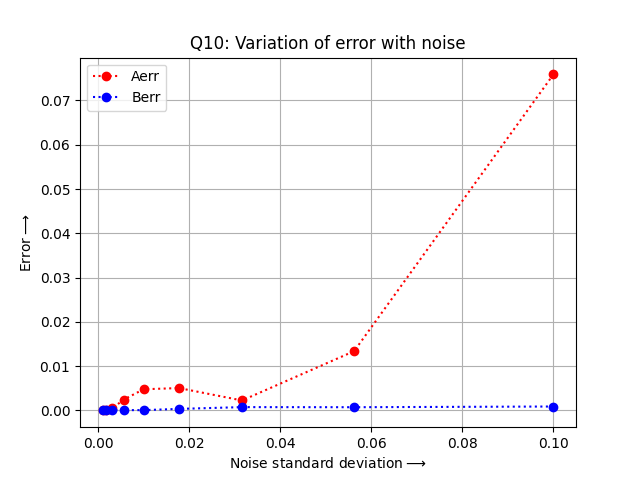
\includegraphics[scale=0.7]{Q10.png}  % Mention the image name within the curly braces. Image should be in the same folder as the tex file. 
   	\caption{A and B error in linear scale}
   	\label{fig:A and B err in linear scale}
\end{figure}
   
The errors in the estimation of A and B are non-linear with respect to $sigma_{n}$

\subsubsection{Loglog scale}
Now we plot the graph in log scale
\begin{lstlisting}
#Function to plot error in loglog scale
def plot_loglog_error(error_A,error_B):
	plt.figure(4)
	plt.grid(True)
	plt.title(r'Q11: loglog Variation of error with noise')
	plt.xlabel(r'Noise standard deviation$\longrightarrow$')
	plt.ylabel(r'loglog Error$\longrightarrow$')
	plt.stem(variance,error_A,'ro')
	plt.stem(variance,error_B,'bo')
	plt.loglog(variance,error_A,'ro-',label='Aerr',linestyle='dotted')
	plt.loglog(variance,error_B,'bo-',label='Berr',linestyle='dotted')
	plt.legend()
	plt.show()

#main
plot_loglog_error(error_A,error_B)
\end{lstlisting}



\begin{figure}[!tbh]
   	\centering
   	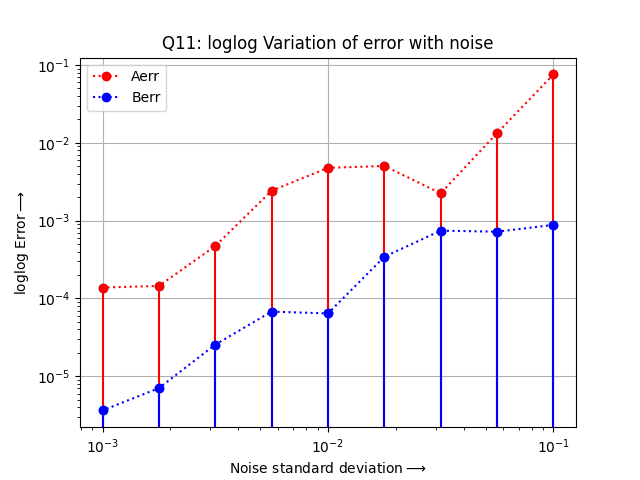
\includegraphics[scale=0.7]{Q11.png}  % Mention the image name within the curly braces. Image should be in the same folder as the tex file. 
   	\caption{A and B error in log scale}
   	\label{fig:A and B err in log scale}
\end{figure}
   
\newpage


\section{Conclusions}
For the given noisy data the best possible estimates for A and B were obtained by minimizing the mean squared error. If we calculate the error for the predicted points w.r.t to the data points, in the log scale we observe that there will be an almost linear variation. This is because the noise we used varied on an algorithmic scale with respect to $\sigma$

 
\end{document}

 